\subsection{Near-ties in calibration utility}
\label{sec:head-intervention}\label{sec:selection-stability}\label{sec:tolerance}
The following diagnostics retain seed 20260910. At complete-sales 220/220, Ratio and Descending have minimum calibration exposure coverages 91.02768\% and 91.00063\%, only 0.02704 points apart; their case coverages differ by 21.83 points (Figure~\ref{fig:near-tie}). Repeating all threshold searches and menu choices on 200 item-cluster resamples selects Ratio/Descending in 51.5\%/48.5\% of draws. Fits, scores, cap and $T$ remain fixed. Changing either head to 660 untuned trees also selects Descending, without consistently improving MSE. These are sensitivity observations, not identified causes or a test of improved moment estimation (Appendices~\ref{app:matched} and \ref{app:v7-stability}).

We examine a retrospective alternative that explicitly values cases within an exposure allowance. Write $\bar c_j=\min_b\widehat c_b(a_j)$ and $\bar d_j=\min_b\widehat d_b(a_j)$ for eligible candidates, and set
\begin{equation}
 \mathcal J_\varepsilon=\{j:\bar d_j\geq\max_k\bar d_k-\varepsilon\},
 \qquad j_{D,\varepsilon}=\mathop{\rm lexargmax}_{j\in\mathcal J_\varepsilon}
 (\bar c_j,\bar d_j).
 \label{eq:tolerance}
\end{equation}
Exact remaining ties use the original fixed order; case selection is unchanged. Positive $\varepsilon$ changes the objective; an exact secondary tie-break cannot resolve a nonzero exposure gap. The illustrative .5-point allowance was recorded before the additional calculation but informed by prior results. It is a utility preference, not a noise estimate or confidence band. Analytic candidate breakpoints show that \emph{every} allowance in [.39,1.63] points selects Ratio in all four complete-sales cells; this contained interval does not justify an operational default (Appendix~\ref{app:v8-tolerance}).

At .5 points, all complete-sales cells select Ratio and all censored cells retain Descending. Relative to the unchanged case choice, this alternative gains 9.63--10.83 exposure points for 10.41--21.23 case points forgone (exchange .454--1.040); headline results retain Equation~\eqref{eq:menu-choice}. Compared with the original exposure choices, three cells gain 13.62--24.11 case points at a .251--.621 exposure-point cost; one cost exceeds the calibration allowance. On the same 200 redesign draws, the complete reference selects Ratio/Mixed/Descending in 97/1.5/1.5\%, whereas Bike selects Ratio/Mixed in 86/14\%, compared with 96/4\% originally. Appendix~\ref{app:v8-tolerance} gives the full grid and interval distributions.

\begin{figure}[t]\centering
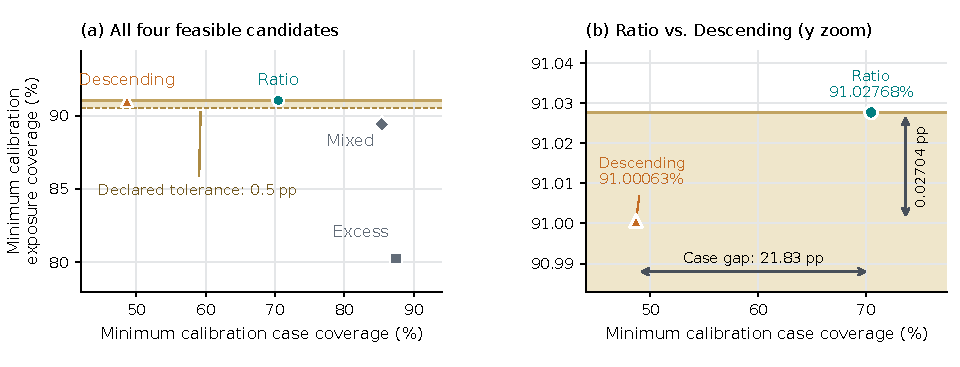
\includegraphics[width=\linewidth]{revision_v8_neartie.pdf}
\caption{Complete-sales 220/220 calibration candidates; Error is infeasible. Minimum case and exposure coverage are taken separately over A/B. The right panel magnifies the exposure axis. Shading marks the illustrative .5-point utility allowance, clipped by the zoom; it is not a confidence interval. Ratio and Descending are close in exposure but far apart in cases.}\label{fig:near-tie}
\end{figure}

\subsection{Separate-window risk evidence and the case floor}
\label{sec:complete-screen}
At fixed complete-sales reporting cap $r=.632683$, thresholds are designed on A at $.95r=.601049$ and checked on B using signed-excess item-bootstrap upper quantiles. Choices maximize A utility among B passers and are frozen before rereading the consumed Later window. At floor .35, all 16 nonempty candidates pass the original 20-candidate screen, and all four head cells select Excess/Descending. Later adjusted risk upper summaries lie below the cap at substantial coverage cost (Appendix~\ref{app:v7-screen}). B removes no candidate; the evidence concerns the combined stricter design and audit.

Descending's maximum A case coverage is only 35.05--35.09\%. Raising the floor to .40 or .45 makes it infeasible and selects Excess/Ratio in all four cells (Table~\ref{tab:v8-floor-main}). Relative to floor .35, the exposure choice gains 9.24--19.02 Later case points and loses 1.17--1.57 exposure points. The exchange persists with a smaller case sacrifice. All 40 nonempty conditions pass the full 60-condition adjustment; the largest selected Later upper summary is .62803, below $r$. These are approximate, fit-conditional summaries with coarse tails. Ratio at 220/660 has only 45.057\% A case coverage, limiting extrapolation beyond the declared floors.

The two designs have different utility gaps: at A-design floor .35, Descending exceeds Ratio by 1.08--1.85 exposure points. The .5-point band leaves all four choices unchanged; with this band, the switch to Ratio requires the higher floor. Holding the floor at .35 instead, a common Ratio choice requires an allowance of at least 1.84693 points (approximately; Appendix~\ref{app:v8-floor} gives both bounds).
\begin{table}[t]\centering\small
\caption{Complete-sales A-design/B-screen floor sensitivity, all four head pairs per row. Ranges show Later exposure-choice minus case-choice coverage (pp), not confidence intervals. $U_{60}$ is the largest approximate upper risk summary among selected conditions, adjusted over all 60 candidate conditions. Fixed reporting cap is .632683; the same selection occurs under the inherited 20-candidate adjustment.}\label{tab:v8-floor-main}
\begin{tabular}{llllr}\toprule
Floor & Case/exposure rules & $\Delta c$ range & $\Delta d$ range & Max. $U_{60}$\\\midrule
0.35 & Excess/Descending & [-36.39, -35.83] & [12.77, 14.29] & 0.62802 \\
0.40 & Excess/Ratio & [-26.78, -16.81] & [11.59, 12.72] & 0.62756 \\
0.45 & Excess/Ratio & [-26.78, -16.81] & [11.59, 12.72] & 0.62756 \\
\bottomrule\end{tabular}\end{table}

